\section{Overview of Grading Methods}
Electric field stress control is important in the design of many power system elements, especially cable terminations and bushings \cite{james2008condition}.
Failure of a bushing can damage the power transformer it is protecting, which can be an expensive mistake \cite{warne2005newnes}.
Bushings are required to withstand Electrical, Mechanical and Thermal stresses as defined in the IEEE standard C57.19.00 \cite{1440990}.
The design of the bushing is largely determined by the insulation material chosen and the resolution of these conflicting sources of stress.
A good bushing design has insulation that can withstand the applied voltage and thermal characteristics appropriate for the current carried by the conductor \cite{harlow2004electric}.

The problem grading methods attempt to resolve is laid out in figure \ref{figure:problem}.
The grounded transformer casing is shown in light grey which is perpendicular to the the bushing insulation shown in dark grey and the high voltage conductor in white.
The top of the bushing is exposed to air, while the other side is exposed to transformer oil.
Conducting a numerical analysis or simulation would show that the conductor surface within the plane of the transformer casing and at the points marked by red crosses would experience high electric field stress.
The bushing insulation is designed to withstand the high electric field between the conductor and the transformer casing, however at the points marked with crosses the interface between the solid insulation and the air/transformer oil would cause surface discharge leading to relatively low flashover voltages \cite{kuffel2000high}.
It is therefore necessary to develop methods of reducing electric field stress to a more uniform distribution for both functional purposes and the economic use of space and materials \cite{james2008condition}.

\begin{figure}[!h]
   \centering
   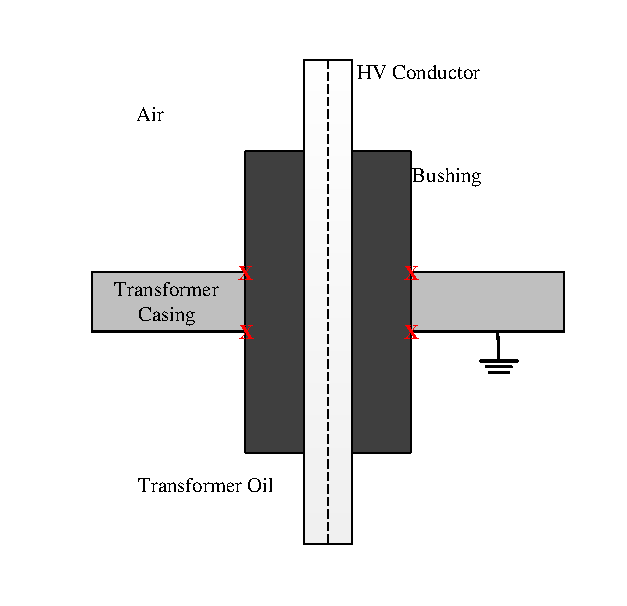
\includegraphics[width = 0.7\textwidth]{GenericBushing.pdf}
   \caption{The Bushing Problem}
   \label{figure:problem}
\end{figure}

\subsection{Low Voltage and DC Solutions}
There are several methods that can be used dependant upon the application.
Low voltage solutions include internal and external screening electrodes, while resistive stress control can be used for DC applications.
\inote{TS - I can't find any good references for these types, only his notes and the hst.tu notes seem to cover it and then it is just lecture slides, not a credible resource like a book or something}

\subsection{Capacitive Grading}
Capacitive grading was first proposed by R.Nagel of Siemens in a German paper published in 1906 \cite{harlow2004electric}.
The value of this type of arrangement was quickly recognised, and is now industry standard practice for AC bushing designs for 25kV - 1500kV applications \cite{james2008condition}.
The general concept of the design is illustrated in figure \ref{figure:fieldgeneric}, showing the isolated foils inserted inside the solid bushing insulation.
Shown in red in figure \ref{figure:fieldgeneric} is the potential field with no grading, and in blue with the isolated conductive foils inserted.
It shows that the whole dielectric is much more evenly stressed with the capacitive grading method.
\begin{figure}[!h]
   \centering
   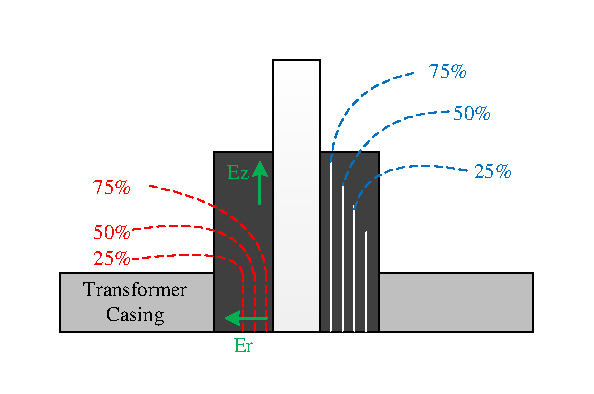
\includegraphics[width = 0.7\textwidth]{BushingFieldDiagram.pdf}
   \caption{Field Distribution both without capacitive grading (shown in red) and with capacitive grading (shown in blue), modified from \cite{james2008condition}}
   \label{figure:fieldgeneric}
\end{figure}

The insulation is stressed in both a radial and axial direction, which sum to give the tangential field.
The radial component $E_r$ can cause breakdown of the insulating material, while the axial component $E_z$ can cause surface discharge along the boundary \cite{Ahmed11}.




